\section{Aufgabe und Ziel des Projektes}
Im Rahmen des Praxisprojektes sollen die ERP-System-Daten der Kunden aus einer externen Quelle (Warenwirtschafts- und ERP-System) standardisiert in die Anwendung von Statistance zur weiteren Auswertung integriert werden können.
Die sich daraus ergebene Aufgabe konnte in mehrere Teilaufgaben aufgesplittet werden. Zunächst können verschiedene Kunden verschiedene ERP-Systeme verwenden. Der Pilotkunde von Statistance nutzt Sage 100 auf welches sich im Rahmen des Projektes fokussiert wurde. Hierbei mussten Möglichkeiten zur Anbindung von Sage 100 gefunden werden. Zukünftig sollen auch andere ERP-Systeme wie Microsoft Dynamics Navision oder Oracle angebunden werden können. Aus diesen Gründen muss die entwickelte Lösung erweiterbar und skalierbar sein. Weiter sollten die aktuellen Daten aus der Quelle des Kunden für Statistance abrufbar sein. Sinnvoll erschien hier die Möglichkeit verschiedener Batch-Jobs, welche von Statistance gesteuert werden können. Daten können hierdurch im unterschiedlichen Turnus abgerufen werden und Statistance mit aktuellen Daten weiter arbeiten. Die sich daraus ergebenen, konkreten Aufgaben sind nachfolgend aufgelistet.
\begin{enumerate}
\item \textbf{Recherche und Auswahl einer geeigneten Technologie}
\item \textbf{Umsetzung} 
\begin{enumerate}
    \item \textbf{API} (Design, Integration, Dokumentation)
    \item \textbf{Integration des ERP-Systems} (Sage 100)
    \item \textbf{Batch-Job} (Scheduling)
    \item \textbf{Security}
    \item \textbf{Config Managament \& API Gateway}
    \item \textbf{Frontend} 
\end{enumerate}
\end{enumerate}

Das Ergebnis des Projektes soll die in \ref{fig:task} dargestellte Lücke zwischen dem Backend von Statistance und dem ERP-System des Kunden schließen.
\begin{figure}[!h]
\centering
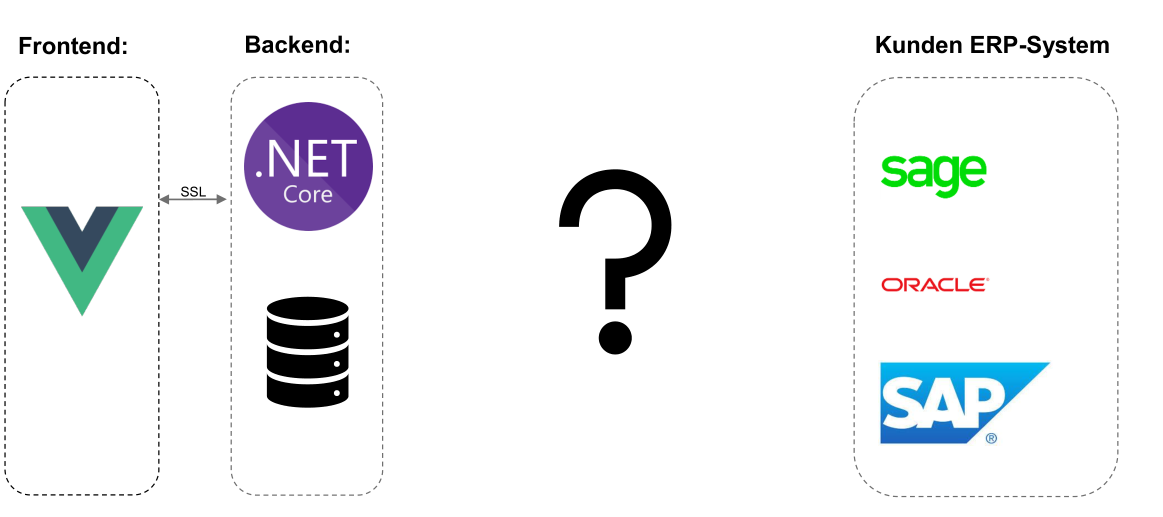
\includegraphics[width=15cm]{images/01_introduction/Aufgabe.PNG}
\caption{Aufgabe}
\label{fig:task}
\end{figure}